\chapter{Introduction to succinct data structures}
\label{kap:kap1}

\section{Motivation}

In many applications, the amount of data is so significant that we optimise how much
space is used by the data structures we use. The field of \textit{succinct data structures}
focuses on representing data using as little space as possible while trying not to hurt
the time complexity and real runtime of methods that these data structures support. In
this field, data structures for many varied problems have been already devised. While
many of these give some solid theoretical bounds on the used space, others look into
real-world space usage and performance.

The most common use case for succinct data structures comes in a situation when we
have a huge amount of data and are trying to implement some useful methods working
with them. The problem we face with regular data structures supporting these
operations is that their representation may not fit into our entire physical
memory. As succinct data structures need to do the work of regular data structures but
with additional constraints on memory usage, the common disadvantage is that
they are often slower and more complicated than their space non-efficient
alternatives. This is mainly because they do more work and at the same time contain
concepts and computation patterns that are slow on modern computers. However, there
are cases in which usage of space-efficient data structures may speed up the overall
running time as they may enable us to store the data in a faster type of memory
(e.g. fast RAM instead of the slower disk). Thus, even if they use slower, more
advanced concepts, the overall runtime may decrease.

%The work in this field turns focus more and more towards the \textit{dynamic succinct
%data structures}. These are structures where the underlying data may change after
%constructing the data structure. However, in this work, we only consider static
%succinct data structures. These are the ones where we get the data, then build
%the succinct data structure and then we support only methods that do not alter the
%underlying data in any way.

In this work, we are mainly concerned about the \textit{bit vector}. One of the simplest
succinct data structures that represents the sequence of zeroes and ones with some
useful method. The reason behind this is that bit vector is one of the main building blocks
of many succinct data structures and can be useful in a lot of use cases. We shall now look
onto some interesting and useful applications of the bit vector. 

\section{Sparse array}

Bit vector can be used to provide us with an implementation of sparse array as was shown
by \cite{grossi2013design}. Let $A$ be an array of $N$ elements. Let us assume that every
element is stored using $k$ bits. To store this array we need in simple case $N\cdot k$ bits
of space. However, imagine a scenario that most of the array is empty, just handful of elements
are filled in. This can be a case for an array of numbers where many of numbers are set to
some default let us say 0 and $n$ of them are arbitrary values. Then we can use a more space
efficient approach. The better approach can be that we only store non-default elements in array
$A'$ of size $n$. Alongside $A'$ we store a bit vector $B$ of size $N$ filled up such that

\[
    B[i]= 
\begin{cases}
	1,& \text{if } A[j]\neq \text{default} \\
    0,& \text{otherwise}
\end{cases}
\].

Using this representation of $A$, if we want to access $i$-th element in $A$, we first check for
the value of $B[i]$. If it is zero, we return the default element. If it is one, we need to find
how many ones are preceding this particular one to know, where in array $A'$ our non-default
value is exactly located. We shall name the number of ones before $i$-th index
$\rank_1(i)$. If we are provided with bit vector implementation along with access and
rank methods we are able to reduce the total space used from $k\cdot N$ to $N+k\cdot n+R$ where
$R$ is space needed to support efficient rank query. If we can make $R$ small, let us say
$R\in o(N)$, this solution shall give us a significant reduction of space used.

\section{Storing elements of non-uniform size}

When trying to optimise the space used, it is often beneficial to use variable-length
code for individual symbols. The example of this is a \textit{Huffman code} that constructs
the code for symbols based on the frequencies with which the symbols occur. This works in a way
that more frequent symbols are assigned bit code that is shorter while less frequent symbols
get a longer code. Although working with these symbols may save space, even storing these
elements and allowing vector like functionality (such as accessing $i$-th element) is not
trivial. Even though we can store these elements one after another in memory, with the
variable-length elements, we do not have an easy and fast way to tell at which offset from the
beginning of the array the $i$-th is element located. Even though there are many solutions, one
of them that is used quite often is using the helper bit vector. Alongside the raw sequence of
bits that store the elements one after another, we create a helper bit vector of the same size.
This bit vector has ones on places where the representation of some element starts and zeroes on
the other places.

Identifying the beginning of $i$-th element now boils down to efficiently finding the
$i$-th one in the helper array. We shall call the method \textit{select} and mark the
answer to this query -- the position of $i$-th one -- $\select_1(i)$. In
Chapter~\ref{kap:kap2}, we shall see how this method can be implemented efficiently.

\begin{figure}
	\centerline{
	\begin{tabular}{l|l|l|l|l|l|l|l|l|l|l|}
	\cline{2-11}
	\textbf{Raw binary representation} & 1          & 1 & 0 & 1 & 1          & 1 & 1          & 0 & 1 & 0          \\ \cline{2-11} 
	\textbf{Helper bit array}          & \textbf{1} & 0 & 0 & 0 & \textbf{1} & 0 & \textbf{1} & 0 & 0 & \textbf{1} \\ \cline{2-11} 
	\end{tabular}
	}
	\caption[TODO]{Raw binary representation of elements 1101, 11, 101 and 0 stored one after another.
	Note the helper bit array that is of the same size with ones on the positions where new element begins.}
	\label{obr:VariableSizedElements}
\end{figure}

\section{FM-index}
% sources to help understand https://www.dcc.uchile.cl/TR/2005/TR_DCC-2005-004.pdf

Let us now consider another practically interesting problem. As we shall see, solution
to this problem also uses bit vector and other building blocks commonly used in succinct
data strucutes. This time, we have a text $T$ and are interested in \textit{indexing} it.
This means if we get some pattern $P$, we would like to quickly answer questions such as
how many times is $P$ contained in $T$ and also where in $T$ this occurrences are located.
This is particularly interesting problem in bioinformatics, where we have very long sequence
of DNA and are interested in searching for some subsequences in it. One of the solutions that
is reasonable and may be used is constructing \textit{suffix array} of $T$. Suffix array is
data structure that for text $T$, stores information about the lexicograpical order of its
suffixes. More precisely, on $i$-th position of suffix array $S$, it stores the starting
position of suffix that comes $i$-th in lexicographical order. Searching for $P$ in suffix
array of $T$ uses fact that if $P$ is contained in $T$ it will be at the beginning of some
suffixes that make up a continuous subsequence of $S$. Succinct data structure that is in
some aspects similar to suffix array was proposed by \cite{ferragina2000opportunistic} and
is called \textit{FM-index}. FM-index can find the pattern in the preprocessed text in time
complexity $\mathcal{O}(|P|)$. On top of this, the resulting space used by FM-index can be
smaller than the space used for the original text $T$. This makes FM-index particularly useful
for searching in very long DNA sequences where FM-index many times takes just 30-40\% of the
space needed for the representation of original text $T$ as was demonstrated by
\cite{ferragina2001experimental}. We shall now look at how the FM-index is obtained for the text
$T$.

\subsection{Burrows-Wheeler transformation}

For simplicity, we assume that the original text $T$ contains a special character {\tt \$}
located at its end that was not contained in $\Sigma$ and is lexicographically smallest.

\textit{Burrows-Wheeler transformation~(BWT)} lies at the heart of the FM-index.
BWT of a text $T$ gives us a sequence $\mathit{T_{BWT}}$ of the same length. Furthermore, this
operation is reversible in a sense that only using $\mathit{T_{BWT}}$ we are able to reconstruct
the original text $T$. This transformation is used as a preprocessing step of some compression
algorithms such as \textit{bzip2} introduced by \cite{seward1996bzip2}. This is because
BWT is oftentimes easier to compress. We shall show how it is constructed and then give 
intuition why it has these properties. We consider the sequence $T$ of symbols over some
alphabet $\Sigma$. Now we take all the cyclical rotations $T_1, T_2, \ldots T_n$ of
the sequence $T$ and imagine putting them sorted by their lexicographical order into the
rows of table $M$ as seen in Fig.~\ref{obr:BWT}. We name the sequence created by the
concatenation of symbols in first and last column $F$ and $L$ respectively. Last column $L$
is what we call the BWT of $T$. Note that the sequence $F$ can be obtained from $L$ just by
sorting all the characters in $\mathit{T_{BWT}}$ and has some nice properties. $F$ consists of
runs of symbols that are sorted according to the lexicographical ordering of alphabet symbols.
We shall use the helper sequence $\mathit{Count}$ where $\mathit{Count}[c]$ is number of
occurrences of symbols smaller than $c$. We note that the run of symbol $c$ in $F$ starts at
the index $\mathit{Count}[c]+1$. We can also see, that the matrix $M$ contains all the suffixes
sorted according to their lexicographical order.

\begin{figure}
	\centerline{
	\begin{tabular}{l|c|ccccc|c|}
	\cline{2-8}
	  & \multicolumn{1}{l|}{\textbf{F}}    & \multicolumn{5}{l|}{}                                                                                                                                                                                                         & \multicolumn{1}{l|}{\textbf{L}}    \\ \cline{2-8} 
	1 & {\color[HTML]{333333} \textbf{\$}} & \multicolumn{1}{c|}{{\color[HTML]{C0C0C0} b}}  & \multicolumn{1}{c|}{{\color[HTML]{C0C0C0} a}}  & \multicolumn{1}{c|}{{\color[HTML]{C0C0C0} n}}  & \multicolumn{1}{c|}{{\color[HTML]{C0C0C0} a}}  & {\color[HTML]{C0C0C0} n}  & {\color[HTML]{000000} \textbf{a}}  \\ \cline{2-8} 
	2 & {\color[HTML]{333333} \textbf{a}}  & \multicolumn{1}{c|}{{\color[HTML]{C0C0C0} \$}} & \multicolumn{1}{c|}{{\color[HTML]{C0C0C0} b}}  & \multicolumn{1}{c|}{{\color[HTML]{C0C0C0} a}}  & \multicolumn{1}{c|}{{\color[HTML]{C0C0C0} n}}  & {\color[HTML]{C0C0C0} a}  & {\color[HTML]{000000} \textbf{n}}  \\ \cline{2-8} 
	3 & {\color[HTML]{333333} \textbf{a}}  & \multicolumn{1}{c|}{{\color[HTML]{C0C0C0} n}}  & \multicolumn{1}{c|}{{\color[HTML]{C0C0C0} a}}  & \multicolumn{1}{c|}{{\color[HTML]{C0C0C0} \$}} & \multicolumn{1}{c|}{{\color[HTML]{C0C0C0} b}}  & {\color[HTML]{C0C0C0} a}  & {\color[HTML]{000000} \textbf{n}}  \\ \cline{2-8} 
	4 & {\color[HTML]{333333} \textbf{a}}  & \multicolumn{1}{c|}{{\color[HTML]{C0C0C0} n}}  & \multicolumn{1}{c|}{{\color[HTML]{C0C0C0} a}}  & \multicolumn{1}{c|}{{\color[HTML]{C0C0C0} n}}  & \multicolumn{1}{c|}{{\color[HTML]{C0C0C0} a}}  & {\color[HTML]{C0C0C0} \$} & {\color[HTML]{000000} \textbf{b}}  \\ \cline{2-8} 
	5 & {\color[HTML]{333333} \textbf{b}}  & \multicolumn{1}{c|}{{\color[HTML]{C0C0C0} a}}  & \multicolumn{1}{c|}{{\color[HTML]{C0C0C0} n}}  & \multicolumn{1}{c|}{{\color[HTML]{C0C0C0} a}}  & \multicolumn{1}{c|}{{\color[HTML]{C0C0C0} n}}  & {\color[HTML]{C0C0C0} a}  & {\color[HTML]{000000} \textbf{\$}} \\ \cline{2-8} 
	6 & {\color[HTML]{333333} \textbf{n}}  & \multicolumn{1}{c|}{{\color[HTML]{C0C0C0} a}}  & \multicolumn{1}{c|}{{\color[HTML]{C0C0C0} \$}} & \multicolumn{1}{c|}{{\color[HTML]{C0C0C0} b}}  & \multicolumn{1}{c|}{{\color[HTML]{C0C0C0} a}}  & {\color[HTML]{C0C0C0} n}  & {\color[HTML]{000000} \textbf{a}}  \\ \cline{2-8} 
	7 & {\color[HTML]{333333} \textbf{n}}  & \multicolumn{1}{c|}{{\color[HTML]{C0C0C0} a}}  & \multicolumn{1}{c|}{{\color[HTML]{C0C0C0} n}}  & \multicolumn{1}{c|}{{\color[HTML]{C0C0C0} a}}  & \multicolumn{1}{c|}{{\color[HTML]{C0C0C0} \$}} & {\color[HTML]{C0C0C0} b}  & {\color[HTML]{000000} \textbf{a}}  \\ \cline{2-8} 
	\end{tabular}
	}
	\caption[TODO]{All the cyclic rotations of sequence $S = \mathit{banana\$}$. BWT is 
	$L$ -- last column. Note that we are not storing this whole table.}
	\label{obr:BWT}
\end{figure}

The reason that BWT is more compressible is that it frequently contains runs of the same
symbol. This can be better explained on an example. Let us create BWT of a text containing
a lot of mentions of word {\tt computer}. All the rotations prefixed with omputer will form a
continuous subsequence of rows of $M$. If we assume, that word {\tt computer} is very frequent
in the text, most of these rows will end in {\tt \$} as this is the most common symbol preceding
word {\tt omputer}. This will for example create the common run of symbol {\tt \$} in BWT.

\subsection{Searching in an FM-index}

As we already stated, FM-index is used for searching in the preprocessed text.
It provides us with the following three methods:

\begin{itemize}
	\item $\mathit{count}(P)$ counts the number of occurrences of $P$ in text $T$
	\item $\mathit{locate}(P)$ returns all positions of pattern $P$ in text $T$
	\item $\mathit{extract}(i, j)$ returns the subsequence $T[i..j]$
\end{itemize}

The reason that the $\mathit{extract}$ method is useful and non-trivial is that FM-index
does not store the original sequence $T$ -- at least not in an easily readable form.

The counting of occurrences of $P$ in $T$ is based on the observation that in $M$,
all the suffix are contained and come in sorted order. Occurrences of $P$ in $M$
are contained in a consecutive subsequence of $M$'s rows. This is the same fact that
enabled searching in suffix array. The search for rows where $P$ is located will proceed
from the end of $P$, gradually by finding rows where $P[n-1..], P[n-2..]$ etc. is located.
At every step, these rows will form a continuous subsequence of rows of $M$ so we will store
only its beginning and end. The process will work in these steps:

\begin{itemize}
	\item We find where $P[n-1]$ is located in $M$. This means setting $b_{n-1}$ to
	$mathit{Count}[P[n-1]]+1$ and $e_{n-1}$ to $\mathit{Count}[P[n-1]+1]$.
	\item Now, to found where $P[n-2..]$ is located in $M$, we would like to locate occurrences
	of $P[n-1]$ that are preceded by $P[n-2]$. In other words, would like to find all
	occurrences of $P[n-2]$ in $L[b_{n-1}..e_{n-1}]$. However, this is not easy to do
	as they can be at arbitrary places in this subsequence, even not in a continuous
	subsequence. Instead of searching in $L$ we look at the occurrences of $P[n-2]$ in
	$F$. Here, they are sorted and it is easy to tell, which of these are followed by
	$P[n-1]$ as $i$-th occurence of character $P[n-1]$ in $L$ corresponds to $i$-th
	occurence of $P[n-1]$ in $F$. Using this fact, we set
	$b_{n-2} = mathit{Count}[P[n-2]] + \rank_{P[n-2]}(b_{n-1})$ and
	$e_{n-2} = mathit{Count}[P[n-2]] + \rank_{P[n-2]}(e_{n-1})$. Here $mathit{Count}[P[n-2]]$
	is the index where run of character $mathit{Count}[P[n-2]]$ starts. $\rank_{P[n-2]}(b_{n-1})$
	is number that gives us number of occurrences of character $Count[P[n-2]]$ in $L$ that
	preceded the index $b_{n-1}$ (starting index of the previous subsequence).
	\item We continue and repeat this process until we compute $b_1$ and $e_1$ or until
	$b_i=e_i$.
\end{itemize}

As we could see, we are not only interested in rank over a bit vector but also over an arbitrary
alphabet that we would like to use in the FM-index. This seems like an even harder task but in
the next section, we shall see, that for a little overhead we can reduce this problem and use
the bit vector implementation also for the rank and select over general alphabet.

\section{Wavelet tree}
\label{section:WaweletTree}

We shall assume for a moment that we have a bit vector implementation supporting
access, rank and select methods. We show how this may be used to create
a more general version of this implementation representing sequence over arbitrary
alphabet still supporting access, rank and select queries in reasonable time complexity.

The most straightforward approach is to store one bit vector of size $|S|$,
per every character of the alphabet $\Sigma$. Let us call these bit vectors $B_1,
B_2, \ldots B_{\sigma}$. Each of them stores one on places where the symbol corresponding
to this bit vector is located, according to the formula

\[
    B_i[j]= 
\begin{cases}
	1,& \text{if } S[j]=i \\
    0,& \text{otherwise}
\end{cases}
\].

This is indeed very fast because we support rank and select in the exact same time
that our bit vector implementation of rank and select is running in. However, we use
roughly $|\Sigma|$ times more space.

\textit{Wavelet tree} uses a divide-and-conquer approach. It takes the sequence $S$ of
length $n$ over some alphabet $\Sigma$ and recursively splits the alphabet into
two subsets creating a hierarchical partitioning of an alphabet. In the root node
of the tree, it splits the alphabet $\Sigma$ into two subsets of the roughly same
size $\Sigma_1, \Sigma_2$. It then stores a bit vector $B$ of size $n$ in this node
where
\[
    B[i]= 
\begin{cases}
    0,& \text{if } S[i]\in \Sigma_1\\
    1,              & \text{otherwise}
\end{cases}
\]

Then it creates two strings $S_1$ and $S_2$ from $S$ by taking just symbols
from $\Sigma_1$ and $\Sigma_2$ respectively. The left and right children of the root node
are then built by recursively applying the same idea on the subsequences $S_1$ and $S_2$.

\begin{figure}
	\centerline{
		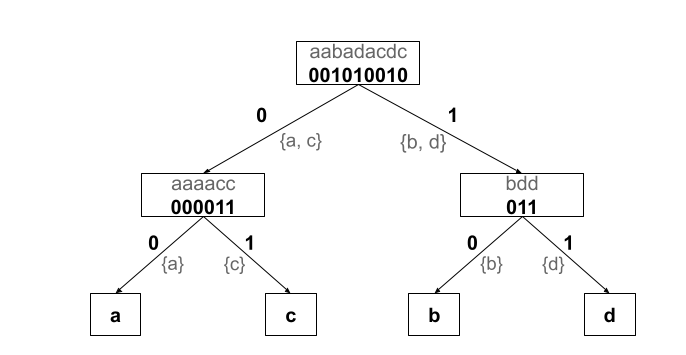
\includegraphics[width=0.9\textwidth, height=0.3\textheight]{images/wavelet_tree}
	}
	\caption[TODO]{Wavelet tree representation of text $S=\mathit{aabadacdc}$. We can see how
	the recursive partitioning of the alphabet works. In every node, we also show the
	subsequence represented (grey text) in the subtree of the node. The stored data can be
	recognized as they are in bold and black.
	}
	\label{obr:WaveletTreeExample}
	% based on https://simongog.github.io/assets/data/sdsl-slides/tutorial#23
	% source at https://docs.google.com/drawings/d/1cJyda3bdTluajr3iXu1x1iL5HF0JPZqAHw6jwct9KLI/edit
\end{figure}

Rank and select methods on the original sequence can be implemented using the tree
traversal and rank/select methods on the individual bit vectors. Another modification
studied by \cite{makinen2005succinct} is to shape the binary tree in a way that a Huffman
tree of the sequence symbols is shaped. Huffman tree is a tree constructed in the
process of creating Huffman encoding of the characters contained in the sequence.

\section{Space efficiency}

There are many ways to measure the space efficiency of a data structure. From the
practical point of view, we may be interested in the memory usage by the data
structure on actual data that the structure could encounter in our use case. However,
many succinct data structures are trying to achieve some upper bounds and express
the used space in terms of the information contained in the data. There are many
models how to measure the information contained in sequences of characters. One
of the most commonly used models in the field of succinct data structures, yet still
quite simple, is entropy or more specifically zeroth-order entropy:

$$H(S)=\sum_{c\in\Sigma} \frac{n_c}{n} \lg \frac{n}{n_c}$$.

In many scenarios, where succinct data structures are used, the stored sequence
is compressible using the sole fact that some symbols have a bigger frequency than others.